\fancyfoot[C]{G�rel}
\paragraph{L�ten mit Reflow-Heizplatte}

Bei dieser L�tmethode wird eine L�tpaste mithilfe einer Schablone auf die Platine aufgetragen. Die Paste besteht gr��tenteils aus Flussmittel und Tr�germaterial, die feine Zinnpartikel enthalten, die in der Fl�ssigkeit verteilt sind. Der Schmelzpunkt betr�gt 140�C und ist schonender f�r die Komponenten. Mit dieser Methode k�nnen Komponenten der Gr��e 0402 und dicht kontaktierte ICs verl�tet werden. Durch die Oberfl�chenspannung des L�tzinns werden die Komponenten bei Erhitzen zentriert auf die Pads gezogen und m�ssen nur selten leicht korrigiert werden.

\begin{figure}[H]
    \centering
    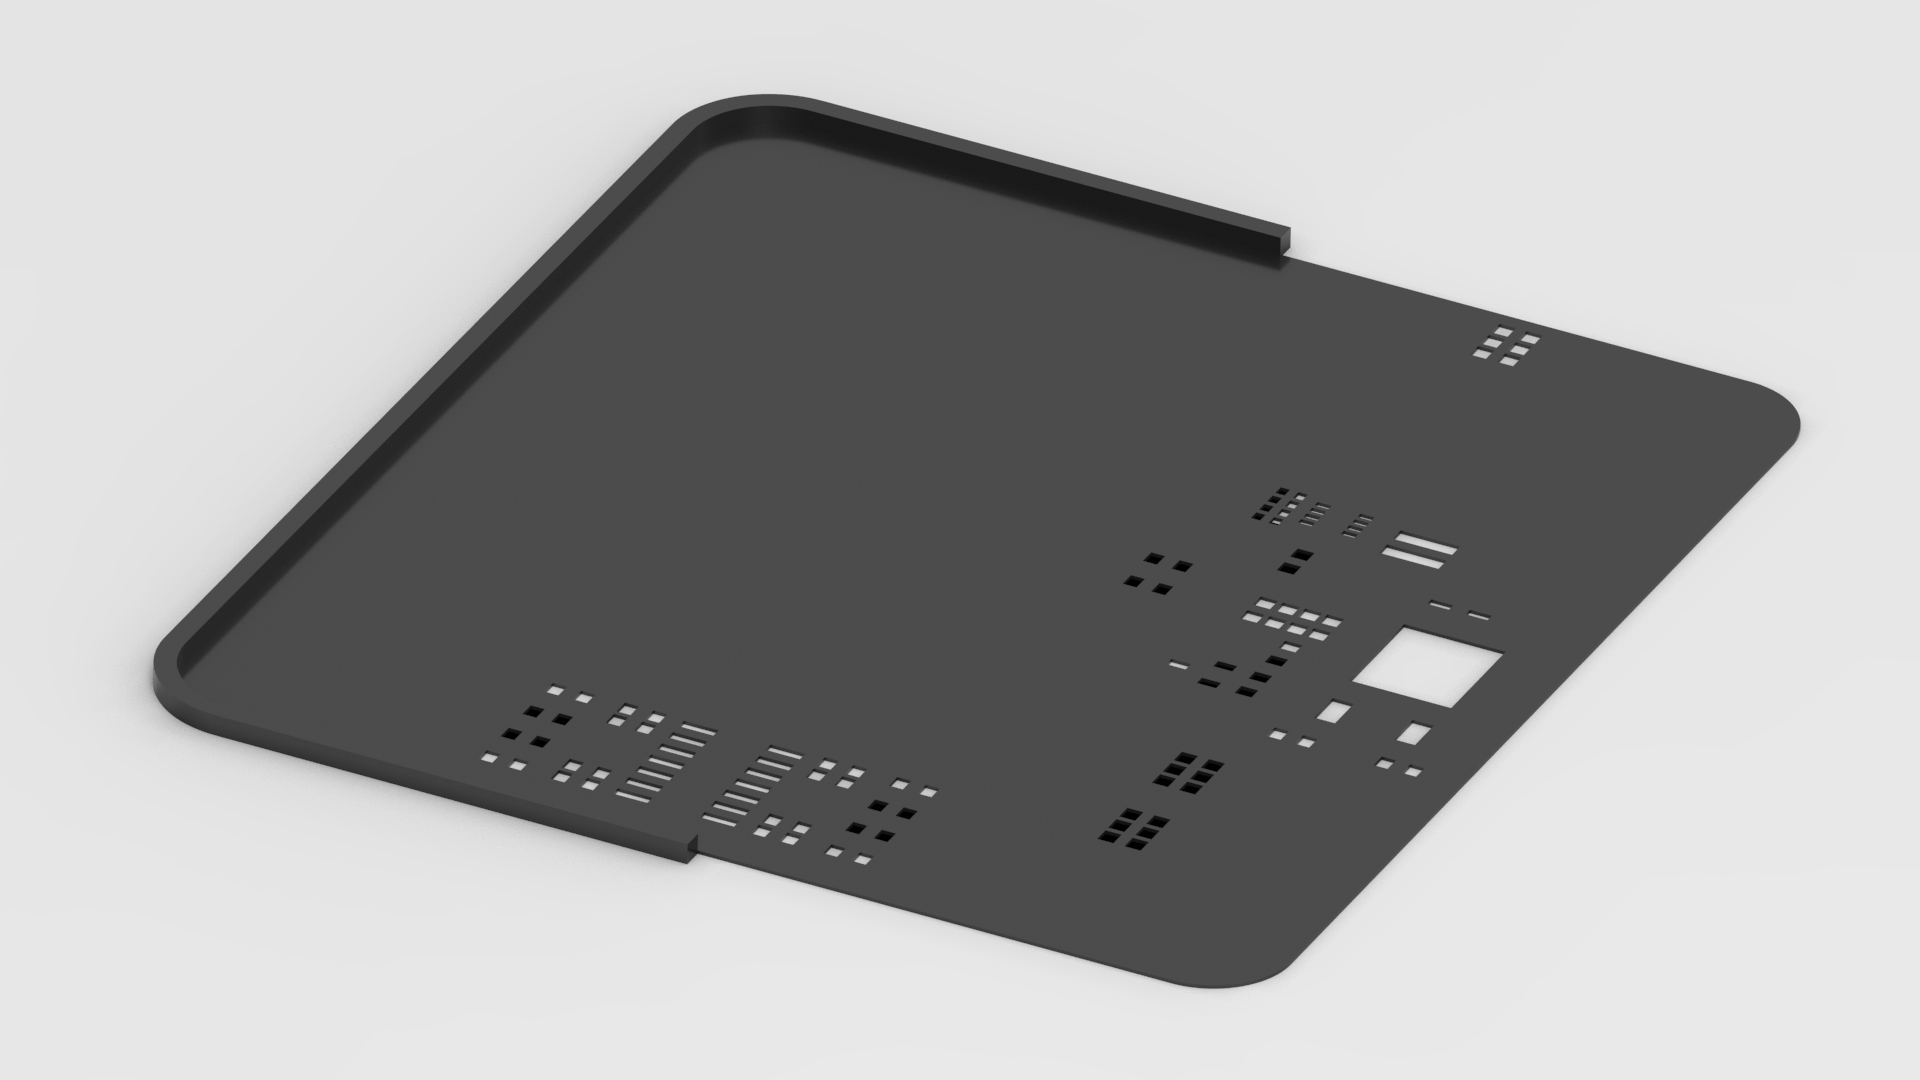
\includegraphics[scale=0.2]{./3_Stand_der_Technik/Abbildungen/stencil.jpg}
    \caption{Symbolfoto Schablone f�r eine Platine \cite{YDLiDAR2024}}
\end{figure}

Die Herstellung und der Versand der Schablone sind kostenintensiv, daher wurde das Online-Tool solder-stencil \cite{Kirberich2016} genutzt. Mit diesem Tool k�nnen Schablonen f�r den 3D-Druck anhand einer Gerber-Datei erstellt werden, welche verschiedene Produktionsdateien wie das Au�enprofil, Bohrungen und Leiterbahnen enth�lt. Dieser erstellt dann eine 3D Datei mit einer festgelegten Dicke und ausschnitte �ber den L�tpads, diese k�nnen mit der Offset Korrektur relativ gesehen kleiner oder gr�sser gemacht werden um die Menge der Paste besser zu regulieren.
